\documentclass{article}

\usepackage{tikz} 
\usetikzlibrary{automata, positioning, arrows} 

\usepackage{amsthm}
\usepackage{amsfonts}
\usepackage{amsmath}
\usepackage{amssymb}
\usepackage{fullpage}
\usepackage{color}
\usepackage{parskip}
\usepackage{hyperref}
  \hypersetup{
    colorlinks = true,
    urlcolor = blue,       % color of external links using \href
    linkcolor= blue,       % color of internal links 
    citecolor= blue,       % color of links to bibliography
    filecolor= blue,        % color of file links
    }
    
\usepackage{listings}
\usepackage[utf8]{inputenc}                                                    
\usepackage[T1]{fontenc}                                                       

\definecolor{dkgreen}{rgb}{0,0.6,0}
\definecolor{gray}{rgb}{0.5,0.5,0.5}
\definecolor{mauve}{rgb}{0.58,0,0.82}

\lstset{frame=tb,
  language=haskell,
  aboveskip=3mm,
  belowskip=3mm,
  showstringspaces=false,
  columns=flexible,
  basicstyle={\small\ttfamily},
  numbers=none,
  numberstyle=\tiny\color{gray},
  keywordstyle=\color{blue},
  commentstyle=\color{dkgreen},
  stringstyle=\color{mauve},
  breaklines=true,
  breakatwhitespace=true,
  tabsize=3
}

\newtheoremstyle{theorem}
  {\topsep}   % ABOVESPACE
  {\topsep}   % BELOWSPACE
  {\itshape\/}  % BODYFONT
  {0pt}       % INDENT (empty value is the same as 0pt)
  {\bfseries} % HEADFONT
  {.}         % HEADPUNCT
  {5pt plus 1pt minus 1pt} % HEADSPACE
  {}          % CUSTOM-HEAD-SPEC
\theoremstyle{theorem} 
   \newtheorem{theorem}{Theorem}[section]
   \newtheorem{corollary}[theorem]{Corollary}
   \newtheorem{lemma}[theorem]{Lemma}
   \newtheorem{proposition}[theorem]{Proposition}
\theoremstyle{definition}
   \newtheorem{definition}[theorem]{Definition}
   \newtheorem{example}[theorem]{Example}
\theoremstyle{remark}    
  \newtheorem{remark}[theorem]{Remark}

\title{CPSC-406 Report}
\author{Nathan Carnnahan  \\ Chapman University}

\date{\today} 

\begin{document}

\maketitle

\begin{abstract}
\end{abstract}

\setcounter{tocdepth}{3}
\tableofcontents

\section{Introduction}\label{intro}

\section{Week by Week}\label{homework}

\subsection{Week 1}
\subsubsection*{HW1 -- DFA Exercises}

\paragraph{Exercise 1}

We are given two DFAs $A_1$ and $A_2$.

\subparagraph{Accepted Words Table}

\begin{center}
\begin{tabular}{c|c|c}
$w$ & Accepted by $A_1$? & Accepted by $A_2$? \\ \hline
aaa & No & Yes \\
aab & Yes & No \\
aba & No & No \\
abb & No & No \\
baa & No & Yes \\
bab & No & No \\
bba & No & No \\
bbb & No & No \\
\end{tabular}
\end{center}

\subparagraph{Language Descriptions}

\begin{itemize}
\item $L(A_1)$: all strings over $\{a,b\}$ that start with $a$ and end with an odd number of $b$'s.
\item $L(A_2)$: all strings over $\{a,b\}$ that end with at least two consecutive $a$'s.
\end{itemize}

\vspace{1em}

\paragraph{Exercise 2 -- Designing DFAs}

\subparagraph{1. Words that end with $ab$}

\begin{center}
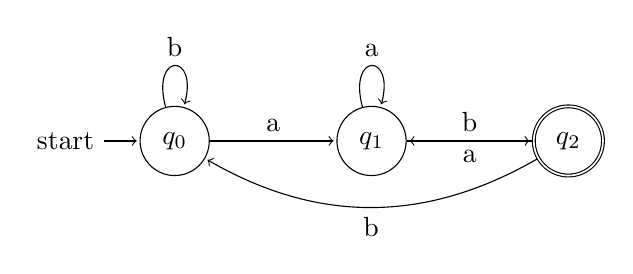
\begin{tikzpicture}[shorten >=1pt,node distance=2.5cm,on grid,auto]
\node[state,initial] (q0) {$q_0$};
\node[state] (q1) [right=of q0] {$q_1$};
\node[state,accepting] (q2) [right=of q1] {$q_2$};

\path[->]
(q0) edge [loop above] node {b} ()
     edge node {a} (q1)
(q1) edge [loop above] node {a} ()
     edge node {b} (q2)
(q2) edge node {a} (q1)
     edge[bend left] node {b} (q0);
\end{tikzpicture}
\end{center}

\subparagraph{2. Words that contain $aba$}

\begin{center}
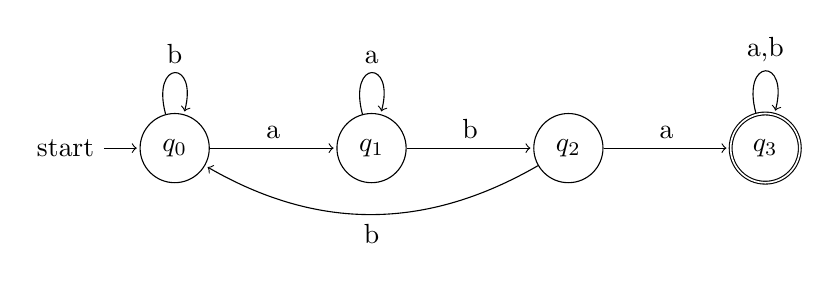
\begin{tikzpicture}[shorten >=1pt,node distance=2.5cm,on grid,auto]
\node[state,initial] (q0) {$q_0$};
\node[state] (q1) [right=of q0] {$q_1$};
\node[state] (q2) [right=of q1] {$q_2$};
\node[state,accepting] (q3) [right=of q2] {$q_3$};

\path[->]
(q0) edge [loop above] node {b} ()
     edge node {a} (q1)
(q1) edge [loop above] node {a} ()
     edge node {b} (q2)
(q2) edge node {a} (q3)
     edge[bend left] node {b} (q0)
(q3) edge [loop above] node {a,b} ();
\end{tikzpicture}
\end{center}

\subparagraph{3. Odd number of $a$'s and odd number of $b$'s}

States represent parity: $(a\text{-parity}, b\text{-parity})$.

\begin{center}
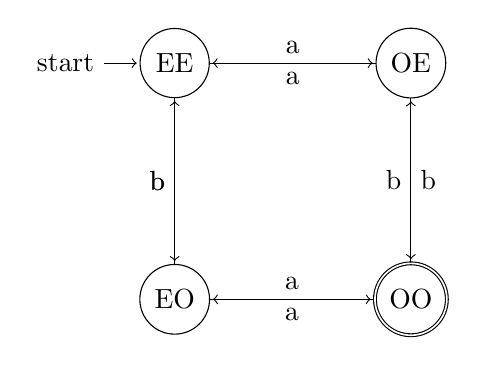
\begin{tikzpicture}[shorten >=1pt,node distance=3cm,on grid,auto]
\node[state,initial] (EE) {EE};
\node[state] (OE) [right=of EE] {OE};
\node[state] (EO) [below=of EE] {EO};
\node[state,accepting] (OO) [right=of EO] {OO};

\path[->]
(EE) edge node {a} (OE)
     edge node[left] {b} (EO)
(OE) edge node {a} (EE)
     edge node {b} (OO)
(EO) edge node {a} (OO)
     edge node {b} (EE)
(OO) edge node {a} (EO)
     edge node {b} (OE);
\end{tikzpicture}
\end{center}

\subparagraph{4. Even number of $a$'s and odd number of $b$'s}

Same automaton as above, but accepting state is EO.

\subparagraph{5. Any three consecutive characters contain at least one $a$}

Equivalent to forbidding substring $bbb$.

\begin{center}
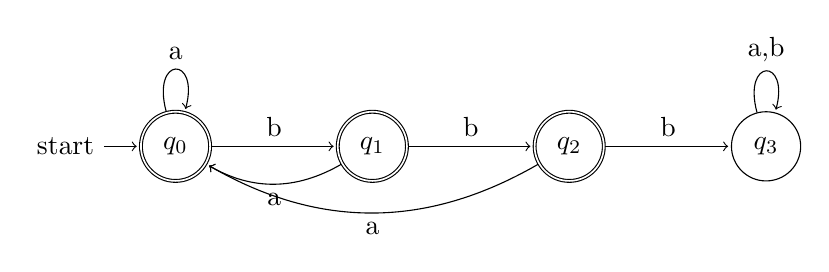
\begin{tikzpicture}[shorten >=1pt,node distance=2.5cm,on grid,auto]
\node[state,initial,accepting] (q0) {$q_0$};
\node[state,accepting] (q1) [right=of q0] {$q_1$};
\node[state,accepting] (q2) [right=of q1] {$q_2$};
\node[state] (q3) [right=of q2] {$q_3$};

\path[->]
(q0) edge node {b} (q1)
     edge[loop above] node {a} ()
(q1) edge node {b} (q2)
     edge[bend left] node {a} (q0)
(q2) edge node {b} (q3)
     edge[bend left] node {a} (q0)
(q3) edge[loop above] node {a,b} ();
\end{tikzpicture}
\end{center}

\subparagraph{6. Words that contain $bbb$}

\begin{center}
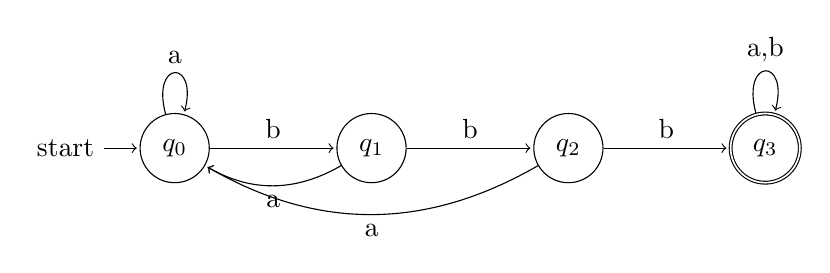
\begin{tikzpicture}[shorten >=1pt,node distance=2.5cm,on grid,auto]
\node[state,initial] (q0) {$q_0$};
\node[state] (q1) [right=of q0] {$q_1$};
\node[state] (q2) [right=of q1] {$q_2$};
\node[state,accepting] (q3) [right=of q2] {$q_3$};

\path[->]
(q0) edge node {b} (q1)
     edge[loop above] node {a} ()
(q1) edge node {b} (q2)
     edge[bend left] node {a} (q0)
(q2) edge node {b} (q3)
     edge[bend left] node {a} (q0)
(q3) edge[loop above] node {a,b} ();
\end{tikzpicture}
\end{center}

\paragraph{Observation}

\begin{itemize}
\item Problems 3 and 4 use the same parity structure; only the accepting state changes.
\item Problems 5 and 6 use the same “count consecutive $b$'s” structure; one treats reaching three $b$'s as rejection, the other as acceptance.
\item Problems 1 and 2 track progress toward matching a pattern.
\end{itemize}


\section{Synthesis}

\section{Evidence of Participation}

\section{Conclusion}\label{conclusion}

\begin{thebibliography}{99}
\bibitem[BLA]{bla} Author, \href{https://en.wikipedia.org/wiki/LaTeX}{Title}, Publisher, Year.
\end{thebibliography}

\end{document}
